\chapter{Tree}

\section{Binary Tree}
\subsection{Introductions}
\runinhead{Get parent ref.} To get a parent reference (implicitly), \textit{return the Node} of the current recursion function to its parent to maintain the path. Sample code:
\begin{java}
Node deleteMin(Node x) {
    if (x.left == null) return x.right;
    x.left = deleteMin(x.left);
    x.count = 1+size(x.left)+size(x.right);
    return x;
}
\end{java}
\runinhead{Construct path from root to target.} To search a node in binary tree (not necessarily BST), use dfs:
\begin{python}
def dfs(self, root, t, path, found):
    if not root or found[0]:  # post-call check
        return

    path.append(root)
    if root == t:
        found[0] = True

    self.dfs(root.left, t, path, found)
    self.dfs(root.right, t, path, found)
    if not found[0]:
        path.pop()  # 1 pop() corresponds to 1 append()
\end{python}
The `found` is a wrapper for boolean to keep it referenced by all calling stack. 

\runinhead{Lowest common ancestor.} In BST, the searching is straightforward. In normal binary tree, construct the path from root to $node_1$ and $node_2$ respectively, and \textbf{diff} the two paths.

\runinhead{Find all paths.} Find all paths from root to leafs. For every currently visiting node, add itself to path; search left, search right and pop itself. Record current result when reaching the leaf.
\begin{python}
def dfs_path(self, cur, path, ret):
    if not cur:
        return

    path.append(cur)
    if not cur.left and not cur.right:
        ret.append("->".join(map(lambda x: str(x.val), path)))

    self.dfs_path(cur.left, path, ret)
    self.dfs_path(cur.right, path, ret)
    path.pop()
\end{python}
 
\section{Binary Search Tree (BST)}
\runinhead{Array and BST.}Given either the \textbf{preorder} or \textbf{postorder} (but not inorder) traversal of a BST containing N distinct keys, it is possible to reconstruct the shape of the BST. 
\subsection{Rank}
\runinhead{Calculates rank.}
\begin{enumerate}
\item When inserting: 
  \begin{enumerate}
  \item insert to an existing node: \pyinline{node.cnt_this += 1}
  \item insert to left subtree: \pyinline{node.cnt_left += 1}
  \item insert to right subtree: do nothing. 
\end{enumerate}
\item When querying rank:
  \begin{enumerate}
  \item query equals current node: \pyinline{return node.cnt_left}
  \item query goes to \textbf{left} node: \pyinline{return rank(node.left, val)};
  \item query goes to \textbf{right} node: \pyinline{return node.cnt_left} \pyinline{+ node.cnt_this + rank(node.right, val)}
  \end{enumerate}
Notice that the \pyinline{rank} calculates a val's rank in a subtree.
\end{enumerate}

\runinhead{Count of smaller number before itself.} Given an array $A$. For each element $A_i$ in the array, count the number of element before this element $A_i$ is smaller than it and return count number array. Average $O(n \log n)$
\\
Clues:
\begin{enumerate}
\item Put $A[:i+1]$ into a BST; so as to count the rank of $A[i]$ in the BST
\end{enumerate}
Codes:
\begin{python}
class Node(object):
  def __init__(self, val):
    """Records the left subtree size"""
    self.val = val
    self.cnt_left = 0
    self.cnt_this = 0
    self.left, self.right = None, None


class BST(object):
  def __init__(self):
    self.root = None

  def insert(self, root, val):
    """
    :return: subtree's root after insertion
    """
    if not root:
      root = Node(val)

    if root.val == val:
      root.cnt_this += 1
    elif val < root.val:
      root.cnt_left += 1
      root.left = self.insert(root.left, val)
    else:
      root.right = self.insert(root.right, val)

    return root

  def rank(self, root, val):
    """
    Rank in the root's subtree
    :return: number of items smaller than val
    """
    if not root:
      return 0
    if root.val < val:
      return (root.cnt_this+root.cnt_left+
              self.rank(root.right, val))
    elif root.val == val:
      return root.cnt_left
    else:
      return self.rank(root.left, val)


class Solution(object):
  def countOfSmallerNumberII(self, A):
    tree = BST()
    ret = []
    for a in A:
      tree.root = tree.insert(tree.root, a)
      ret.append(tree.rank(tree.root, a))

    return ret
\end{python}
Notice: if worst case $O(n \log n)$, need to use Red-Back Tree.


\subsection{Range search}
\runinhead{1-d range count}
\begin{java}
int size(Key lo, Key hi) {
    if (contains(hi)) return rank(hi)-rank(lo)+1;
    else              return rank(hi)-rank(lo);
}
\end{java}
\runinhead{1-d range search}
TODO

\runinhead{Closest value} Find the value in BST that is closet to the \pyinline{target}.

Clues:
\begin{enumerate}
\item Find the value just $\leq$ the target.
\item Find the value just $\geq$ the target.
\end{enumerate}

Code for finding either the lower value or higher value:
\begin{python}
def find(self, root, target, ret, lower=True):
  if not root:
    return

  if root.val == target:
    ret[0] = root.val
    return

  if root.val < target:
    if lower:
      ret[0] = max(ret[0], root.val)

    self.find(root.right, target, ret, lower)
  else:
    if not lower:
      ret[0] = min(ret[0], root.val)

    self.find(root.left, target, ret, lower)
\end{python}

\runinhead{Closet values} Find $k$ values in BST that are closet to the \pyinline{target}.

Clues:
\begin{enumerate}
\item Find the predecessors $\triangleq \{node | node.value \leq target\}$.
\item Find the successors $\triangleq \{node | node.value \geq target\}$.
\item Merge the predecessors and successors as in merge in MergeSort to get he $k$ values. 
\end{enumerate}

Code for finding the predecessors:
\begin{python}
def predecessors(self, root, target, stk):
  if not root:
    return

  self.predecessors(root.left, target, stk)
  if root.val <= target:
    stk.append(root.val)
    self.predecessors(root.right, target, stk)
\end{python}




\section{Binary Index Tree (BIT)}\label{BIT}
Given an array $A$ of length $n $ starting from $1$. prefix sum $s[i]\triangleq A_1+...+A_i$. BIT uses binary to maintain the array of prefix sum for querying and updating. For $i$-th node in the BIT, 
$$
N[i]=A_{j+1}+...+A_i
$$
, where $j=i-lowbit(i)$, i.e. set $i$'s lowest bit 1 to 0. $lowbit(i)$ can be defined as \pyinline{return i&-i}, using 2's complement. 
\\
Clues:
\begin{enumerate}
\item Binary 
\item Low bit
\item BIT uses array index starting from \textbf{1}, because 0 doesn't have $lowbit$.
\end{enumerate}
\begin{figure}[hbtp]
\centering
\subfloat{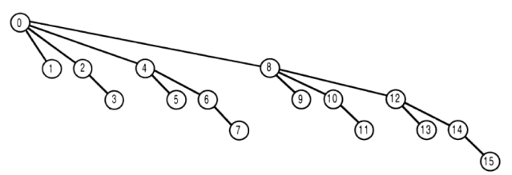
\includegraphics[height=1.1in]{BITget}}
\caption{Binary Indexed Tree Get Operation}
\label{fig:LABEL}
\end{figure}

\begin{figure}[hbtp]
\centering
\subfloat{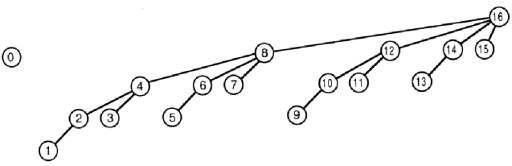
\includegraphics[height=1.05in]{BIT}}
\caption{Binary Indexed Tree Set Operation}
\label{fig:LABEL}
\end{figure}

Time complexity, longest update is along the leftmost branch, which takes $O(\log_2 n)$ (e.g. 1, 10, 100, 1000, 10000); longest query is along a branch starting with node with all 1's (e.g. 1111, 1110, 1100, 1000), which also takes $O(\log_2 n)$.\\
Code:
\begin{python}
class BIT(object):
    def __init__(self, n):
        """BIT uses index starting from 1"""
        self.N = [0 for _ in xrange(n+1)]

    def lowbit(self, i):
        return i & -i

    def set(self, i, val):
        while i < len(self.N):
            self.N[i] += val
            i += self.lowbit(i)

    def get(self, i):
        ret = 0
        while i > 0:
            ret += self.N[i]
            i -= self.lowbit(i)

        return ret
\end{python}


\section{Segment Tree}
\subsection{Introduction}
The structure of \textbf{Segment Tree} is a binary tree which each node has two attributes start and end denote an segment/interval. 

Notice that by practice, the interval is normally $[start, end)$ but sometimes it can be $[start, end]$, which depends on the question definition. 

Structure:  
\begin{lstlisting}[columns=flexible]
# a Count Segment Tree
                     [0, 4, count=3]
                     /             \
          [0,2,count=1]             [2,4,count=2]
          /         \               /            \
   [0,1,count=1] [1,2,count=0] [2,3,count=1], [3,4,count=1]
\end{lstlisting}

Variants:
\begin{enumerate}
\item Sum Segment Tree.
\item Min/Max Segment Tree.
\item Count Segment Tree. 
\end{enumerate}

For a \textbf{Maximum Segment Tree}, which each node has an extra value max
to store the maximum value in this node's interval.

\subsection{Operations}
Components in Segment Tree:
\begin{enumerate}
\item Build
\item Query 
\item Modify
\item Search 
\end{enumerate}
Notice:
\begin{enumerate}
\item Only build need to change the start and end recursively.
\item Pre-check is preferred in recursive calls.
\end{enumerate}


Code:
\begin{python}
DEFAULT = 0
f = lambda x, y: x+y


class Node(object):
    def __init__(self, start, end, m):
        self.start, self.end, self.m = start, end, m
        self.left, self.right = None, None


class SegmentTree(object):
    def __init__(self, A):
        self.A = A
        self.root = self.build_tree(0, len(self.A))

    def build_tree(self, s, e):
        """
        segment: [s, e)
        """
        if s >= e:
            return None

        if s+1 == e:
            return Node(s, e, self.A[s])

        left = self.build_tree(s, (s+e)/2)
        right = self.build_tree((s+e)/2, e)

        val = DEFAULT
        if left: val = f(val, left.m)
        if right: val = f(val, right.m)
        root = Node(s, e, val)
        root.left = left
        root.right = right

        return root

    def query(self, root, s, e):
        """
        :type root: Node
        """
        if not root:
            return DEFAULT

        if s <= root.start and e >= root.end:
            return root.m

        if s >= root.end or e <= root.start:
            return DEFAULT

        l = self.query(root.left, s, e)
        r = self.query(root.right, s, e)
        return f(l, r)

    def modify(self, root, idx, val):
        """
        :type root: Node
        """
        if not root or idx >= root.end or idx < root.start:
            return

        if idx == root.start and idx == root.end-1:
            root.m = val
            self.A[idx] = val
            return

        self.modify(root.left, idx, val)
        self.modify(root.right, idx, val)

        val = DEFAULT
        if root.left:  val = f(val, root.left.m)
        if root.right: val = f(val, root.right.m)
        
        root.m = val
\end{python}
Concrete example - Count Segment Tree \ref{inversionReconstruct}. 
        
     
